%%----------------------------------------------------------------------
%%----------------------------------------------------------------------
\missiontitle{Mission: Open Ground}

\teaser{In war, two armies cannot stand together, and yet they cannot
  stay apart.}

\begin{tablesetup}    
  \dawnofwar

  \smallskip%
  Place six primary objective markers in two lines of three.  On a 4'
  x 4' board the lines are to be 12'' from each short table edge, on a
  4' x 6' they are to be 18'' from each short table edge.  Two markers
  are placed at 12'' from each long table edge and the third on the
  table center line, as shown below for 4' x 4'.

  \hfill
  \begin{minipage}[t]{2.5in}\vbox to 0pt{}
  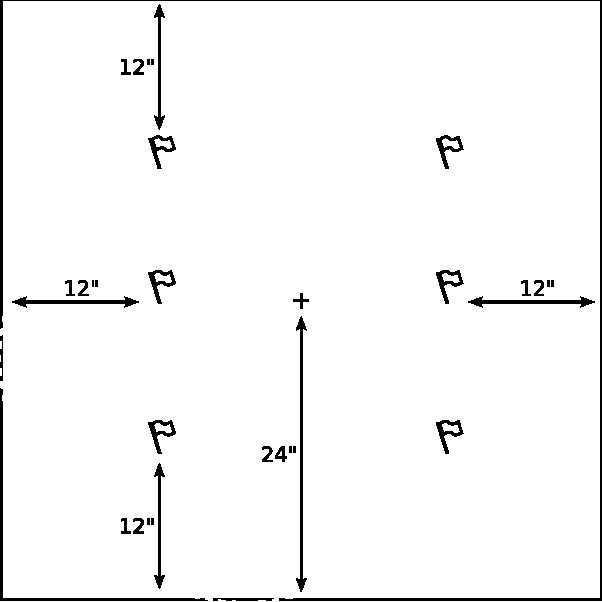
\includegraphics[width=\linewidth]{missions/ground-placement}
  \end{minipage}
  \hfill\hbox to 0pt{}

\end{tablesetup}

%%----------------------------------------------
\begin{missionrules}

\bigskip
There are no rules specific to this mission.

\end{missionrules}


%%----------------------------------------------
\begin{scoring}

\begin{primaries}
  Before any Scout redeployments, both players secretly choose one of
  the following primary scoring mechanisms for themselves:

  \begin{itemize}
  \item {\textit{Continuous.}} Beginning with Turn~2, score~1 victory
    point at the end of each of your player turns for each primary
    objective marker you control.
  
  \item {\textit{End Game.}} At game end, score~3 victory points for
    each primary objective marker you control.
  
  \end{itemize}

  This selection is declared along with the choice of secondary
  objective, below, after Scout redeployments.  Remember that
  \underline{no more than 9 victory points may be earned toward
    primary objectives}.  
\end{primaries}

\end{scoring}
